% Include from the project root; requires graphicx and amsmath.
\begin{figure*}[t]
  \centering
  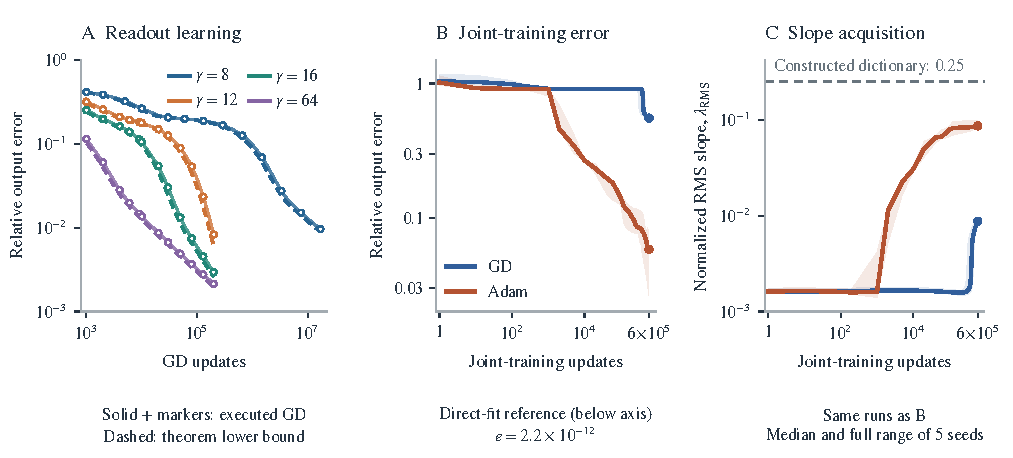
\includegraphics[width=\textwidth]{output/pdf/paper_training_failure_three_panel.pdf}
  \caption{\textbf{Slope scale controls readout learning, while joint training falls short of a constructed reference.}
  \textbf{(A)} Executed frozen-feature GD (solid lines and markers) and theorem-derived output-error lower bounds (dashed), with fixed centers and common slopes $\gamma\in\{8,12,16,64\}$.
  The bounds use gamma-dependent rate enclosures and actual target projections, without fitting to training trajectories.
  \textbf{(B)} Raw output error during joint GD and Adam training. Lines show seed medians; shading shows the full range of five paired seeds.
  The same-width constructed dictionary with a directly fitted readout achieves $2.20\times10^{-12}$ error, annotated below the plotted range.
  \textbf{(C)} Normalized RMS slope $\lambda_{\mathrm{RMS}}=h\sqrt{W^{-1}\sum_j a_j^2}$ at the same checkpoints as B; the dashed line marks the constructed dictionary's scale, $0.25$.
  Error is $\|f-y\|_2/\|y\|_2$ on each experiment's training grid.
  A uses $W=559$, 8,193 samples and $f_5$; B/C use $W=177$, 2,048 samples and the RMS-normalized $f_7$, where $f_k(x)=\sin(2\pi x)+\tfrac12\sin(6\pi x)+\tfrac14\sin(2k\pi x)$.
  Bounds are checked FP64 evaluations. The frozen-feature theorem does not assert an Adam convergence law; C's reference is a construction benchmark, not a universal slope threshold.}
  \label{fig:slope-training-failure}
\end{figure*}
